%%% Template originaly created by Karol Kozioł (mail@karol-koziol.net) and modified for ShareLaTeX use
%%% lionel.rou.durand@ensae.fr
\documentclass[a4paper,11pt]{article}

\usepackage{listings}
\usepackage{lmodern}
\usepackage{amsmath,amssymb,amsthm,textcomp}
\usepackage[utf8]{inputenc}  
\usepackage[T1]{fontenc}  
\usepackage{ listings }
\usepackage{graphicx}
\usepackage{float}
\usepackage{enumitem}
\usepackage{bbm}
\graphicspath{ {images/} }

\usepackage{geometry}
\geometry{total={210mm,297mm},
left=15mm,right=15mm,%
bindingoffset=0mm, top=20mm,bottom=20mm}

\usepackage{etoolbox}
\makeatletter
\preto{\@verbatim}{\topsep=0pt \partopsep=3pt }
\makeatother

\linespread{1}

\newcommand{\linia}{\rule{\linewidth}{0.5pt}}


% my own titles
\makeatletter
\renewcommand{\maketitle}{
\begin{center}
\vspace{2ex}
{\huge \textsc{\@title}}
\vspace{1ex}
\\
\linia\\
\@author 
\vspace{4ex}
\end{center}
}
\makeatother
%%%

% custom footers and headers
\usepackage{fancyhdr}
\pagestyle{fancy}
\lhead{}
\chead{}
\rhead{}

\cfoot{}
\rfoot{Page \thepage}
\renewcommand{\headrulewidth}{0pt}
\renewcommand{\footrulewidth}{0pt}
%
\DeclareMathOperator*{\argmax}{arg\,max}
\DeclareMathOperator*{\argmin}{arg\,min}

%%%----------%%%----------%%%----------%%%----------%%%

\begin{document}

\title{HW3}

\author{Gabriel ROMON}



\maketitle

\section*{1}

In order to turn the problem into a constrained one, we add an auxiliary variable $z\in \mathbb R^n$: $$\min_{w,z} \frac 12 \|z\|_2^2 + \lambda \|w\|_1 \quad \text{s.t} \quad z = Xw-y$$

The Lagrangian of this problem is $\displaystyle L\left(\begin{pmatrix}w\\z \end{pmatrix}, \nu\right) = \frac 12 \|z\|_2^2 + \lambda \|w\|_1 + \nu^T(z-Xw+y)$.\newline
For a fixed $\nu$, note that $$\begin{aligned}\inf_{w,z} L\left(\begin{pmatrix}w\\z \end{pmatrix}, \nu\right) 
&= \inf_{w,z} \left[\frac 12 \|z\|_2^2 + \lambda \|w\|_1 + \nu^T(z-Xw+y) \right] \\
&= \inf_z \left[ \frac 12 \|z\|_2^2 + \nu^Tz  + \inf_w(\lambda \|w\|_1 - \nu^TXw)\right] + \nu^Ty\\
&= \inf_z \left[ \frac 12 \|z\|_2^2 + \nu^Tz  -\lambda \sup_w(\frac{1}{\lambda}(X^T\nu)^Tw - \|w\|_1 )\right] + \nu^Ty\\
&= \inf_z \left[ \frac 12 \|z\|_2^2 + \nu^Tz  -\lambda f^*(\frac{1}{\lambda}X^T\nu)\right] + \nu^Ty
\end{aligned}$$ 
where $f^*$ is the conjugate of the $\|\cdot\|_1$ function. $f^*$ has already been computed in HW2 so we skip its derivation.

Hence $$\begin{aligned}\inf_{w,z} L\left(\begin{pmatrix}w\\z \end{pmatrix}, \nu\right) 
&= \begin{cases}\inf_z \left[ \frac 12 \|z\|_2^2 + \nu^Tz \right] + \nu^Ty &\text{if} \quad \|X^T\nu\|_{\infty} \leq \lambda \\
-\infty &\text{otherwise}
\end{cases}
\end{aligned}$$ 

\noindent $z\mapsto \frac 12 \|z\|_2^2 + \nu^Tz$ is a convex differentiable function, and is thus minimized at a critical point. We find that $z=-\nu$ is a critical point, hence $\inf_z \left[ \frac 12 \|z\|_2^2 + \nu^Tz \right] = -\frac 12 \|\nu\|_2^2$ and finally 

$$\begin{aligned}\inf_{w,z} L\left(\begin{pmatrix}w\\z \end{pmatrix}, \nu\right) 
&= \begin{cases} -\frac 12 \|\nu\|_2^2 + \nu^Ty &\text{if} \quad \|X^T\nu\|_{\infty} \leq \lambda \\
-\infty &\text{otherwise}
\end{cases}
\end{aligned}$$ 

\noindent The dual problem of LASSO is therefore $$\max_{\nu} -\frac 12 \|\nu\|_2^2 + \nu^Ty \quad \text{s.t} \quad \|X^T\nu\|_{\infty}\leq \lambda$$
Since $\|X^T\nu\|_{\infty}\leq \lambda \iff \begin{pmatrix}X^T \\ -X^T \end{pmatrix} \nu \leq \lambda \mathbf 1_{2d}$, the problem rewrites as 
$$\max_{\nu} -\frac 12 \nu^TI_n\nu  + y^T \nu \quad \text{s.t} \quad \begin{pmatrix}X^T \\ -X^T \end{pmatrix} \nu \leq \lambda \mathbf 1_{2d}$$ and it suffices to solve 
$$\min_{\nu} \frac 12 \nu^TI_n\nu  - y^T \nu \quad \text{s.t} \quad \begin{pmatrix}X^T \\ -X^T \end{pmatrix} \nu \leq \lambda \mathbf 1_{2d}$$
which turns into the Quadratic Problem 
$$\min_{\nu} \nu^TQ\nu  + p^T \nu \quad \text{s.t} \quad A \nu \leq \lambda b$$
with $$ Q=\frac 12 I_n, \quad p=-y, \quad A = \begin{pmatrix}X^T \\ -X^T \end{pmatrix},\quad  b=\lambda \mathbf 1_{2d}$$

\section*{2}
Our implementation of the barrier method is the strict Python transcription of the algorithms in Boyd's book. For our case, it is important to note that there are no equality constraints, so we may use Newton's unconstrained minimization method for the centering steps.\newline
Throughout the code, we let $$f_t:\nu \mapsto t(\nu^TQ\nu  + p^T) - \sum_{i=1}^d \log(b_i-L_i \nu)$$ where $L_i$ is the $i$-th line of $A$. For the Newton step it is necessary to compute the gradient and Hessian of $f_t$, which are given by $$\begin{aligned}[t]\nabla f_t(\nu) &= t((Q+Q^T)\nu + p) + \sum_{i=1}^{2d} \frac{1}{b_i-L_i\nu}L_i^T\\
H(f_t)(\nu) &= 2tQ + \sum_{i=1}^{2d} \frac{1}{(b_i-L_i\nu)^2}L_i^TL_i\end{aligned}$$
The step size in Newton's method is obtained by backtracking line search.
\newline \newline 
\noindent The parameters of the method can be decomposed as follows: 
\begin{itemize}
  \item in the line search: $\alpha\in \left(0,\frac 12 \right)$ and $\beta\in (0,1)$
  \item in Newton's method: a tolerance $\varepsilon_{\text{Newton}}$
  \item in the barrier method: an initial $t^{(0)}>0$, a tolerance $\varepsilon_{\text{barrier}}$, and $\mu> 1$
\end{itemize}

\section*{3}

We set arbitrary values of the aforementioned parameters and we work with dimensions $d=50$, $n=10$. The results of the method for a randomly generated $X$ and $y$ are displayed in Figure 1. A trade-off can be observed according to the value of $\mu$. If $\mu$ is small ($\mu=2$ in this example), there is a small number of Newton steps (inner iterations) per outer iteration, which is counterbalanced by a large number of outer iterations. When $\mu$ is large ($\mu=300$ here), there are more inner iterations and less outer iterations. \newline
A balance between the two is reached for $\mu=50$, which corresponds to the green curve in Figure 1. 
\begin{figure}[H]
\centering
 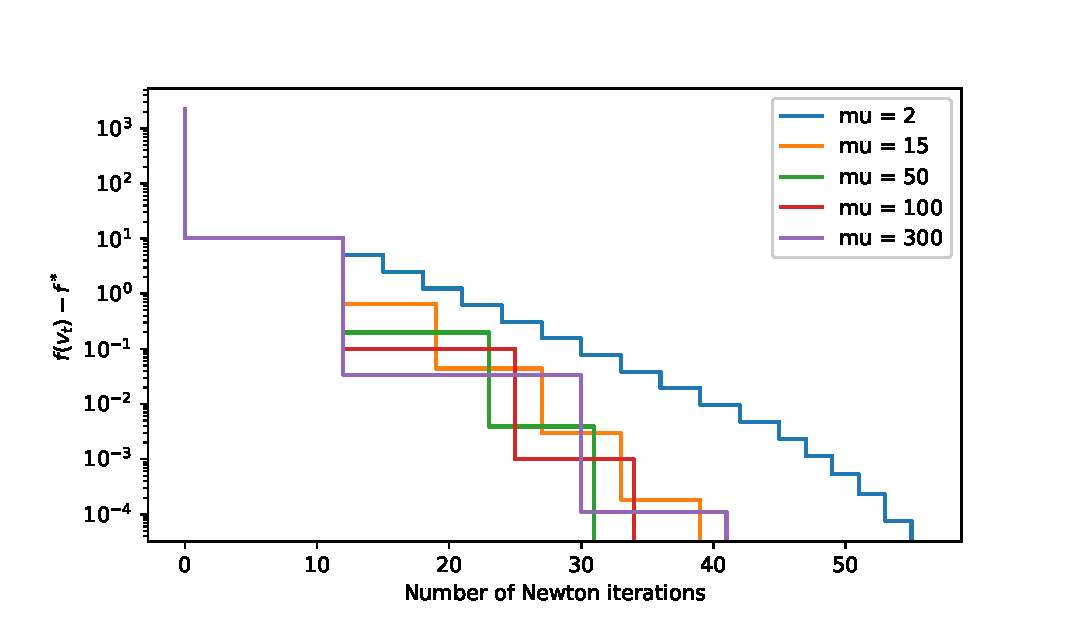
\includegraphics[scale=0.7]{plot.eps}  \\
\caption{Progress of barrier method, showing approximate duality gap versus cumulative number of Newton steps, for different $\mu$'s}
\end{figure}


\end{document}